% !TeX root = ./Skript_DB.tex
\cohead{\Large\textbf{DBMS und SQL}}
\section[DBMS und SQL]{Datenbankmanagementsystem und Structured Query Language}
\subsection{Begriffe}
In einer Datenbank werden die Daten oder auch Informationen abgelegt. Für das Erstellen oder Ändern der Daten oder auch für die Abfrage von Daten benötigt man ein Programm, das sogenannte Datenbankmanagementsystem. So wie es verschiedene Tabellenkalkulationsprogramme wie z.B. Excel, Calc oder Numbers gibt, gibt es auch verschiedene DBMS, z.B. Oracle, Postgres oder DB2.

Obwohl es kleinere Unterschiede vor allem im Design der Oberfläche gibt, funktionieren alle Tabellenkalkulationsprogramme in großen Teilen gleich, z.B. summiert \lstinline!SUM(A1; B3; C5)! die Werte der angegebenen Zellen zusammen. Etwas ähnliches gibt es für DBMS ebenfalls. Fast alle DBMS verwenden SQL bzw. Structured Query Language für das Verwalten der Datenbank. Will man z.B. eine neue Tabelle in der Datenbank erstellen, so kann man nicht einfach auf \textit{Neu} in einer Oberfläche klicken, so wie man z.B. in Word ein neues Dokument erstellen kann, sondern muss dem DBMS eine Anweisung in Textform als SQL-Befehl geben, wie z.B.
 \lstinline!CREATE TABLE farben(laufendeNR INT PRIMARY KEY, bezeichnung TEXT,!

\lstinline!rotanteil INT NOT NULL, blauanteil INT NOT NULL, gruenanteil NOT NULL);!.

Ein sehr entfernt ähnliches Konzept haben bei HTML mit den verschiedenen Tags kennengelernt.

SQL selbst ist nicht case sensitive, d.h. die Groß- und Kleinschreibung spielt keine Rolle. Jedoch hat es sich eingebürgert die SQL-Schlüsselwörter komplett in Großbuchstaben zu schreiben und die Bezeichnungen von Tabellen/Entitäten und Attributen klein zuschreiben. Jeder SQL-Befehlt endet mit einem Strichpunkt.

Wir werden als DBMS SQLite verwenden, da es nicht viel Speicherplatz braucht und es eine portable Version gibt, d.h. es ist keine Installation notwendig. SQLite kann man starten, indem man die \texttt{sqlite3.exe} startet.

\begin{figure}[h]
	\centering
	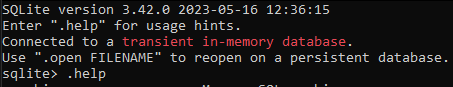
\includegraphics[]{\pics/sqliteStart.png}
	\caption*{Kommandozeile nach dem Starten von \texttt{sqlite3.exe}.}
\end{figure}
Alle SQLite-Befehle beginnen mit einem Punkt. Für Interessierte: Der Befehl \lstinline!.help! gibt eine Übersicht der möglichen Befehle. Wir werden aber nur wenige Befehle, wie z.B. \lstinline!.open bsp.db! verwenden.